\documentclass[11pt, leqno]{article}
\usepackage[utf8]{inputenc}

\usepackage{amsmath,amssymb,amsthm}
\renewcommand{\theequation}{\alph{equation}}
\usepackage[pdftex]{graphicx}
\usepackage[shortlabels]{enumitem}
\usepackage[inline]{asymptote}
\usepackage{fancyhdr}
\usepackage{mathtools}
\usepackage[english]{babel}
\usepackage[margin=.75 in]{geometry}
\usepackage[nottoc]{tocbibind}
\usepackage{hyperref}
\usepackage{setspace}
\usepackage{csquotes}
\usepackage[style=mla-new]{biblatex}
\usepackage[final]{pdfpages}
\usepackage[version=4]{mhchem}
\usepackage{siunitx}

\usepackage{empheq}
\newcommand{\standard}{^\circ}
\pagestyle{fancy}
\lhead{Class Diagnostic}
\rhead{\thepage}


\begin{document}
\begin{center} \LARGE \textbf{CaMO USNCO Local Exam Pre-Test} \end{center}
\begin{center}
    Local Section Diagnostic
\end{center}
\begin{center} Vishal Canumalla \end{center}


 \noindent Rules: You have 50 minutes to complete this 27 question multiple choice exam. You may use a non programmable calculator. You are not allowed to access the internet during this exam. I will not aid you during this exam. \\
 
 \centering\textbf{DO NOT TURN THE PAGE UNTIL DIRECTED TO DO SO}

\begin{center}

    \begin{align*}
        E = E^{\circ} - \frac{RT}{nF}\ln{Q} && \ln{K} = \left(\frac{-\Delta{H^{\circ}}}{R}\right)\left(\frac{1}{T}\right) + \text{constant} && \ln \left({\frac{k_2}{k_1}}\right) = \frac{E_a}{R}\left(\frac{1}{T_1} - \frac{1}{T_2}\right)
    \end{align*}
    

\end{center}
%\hspace{-0.69 in}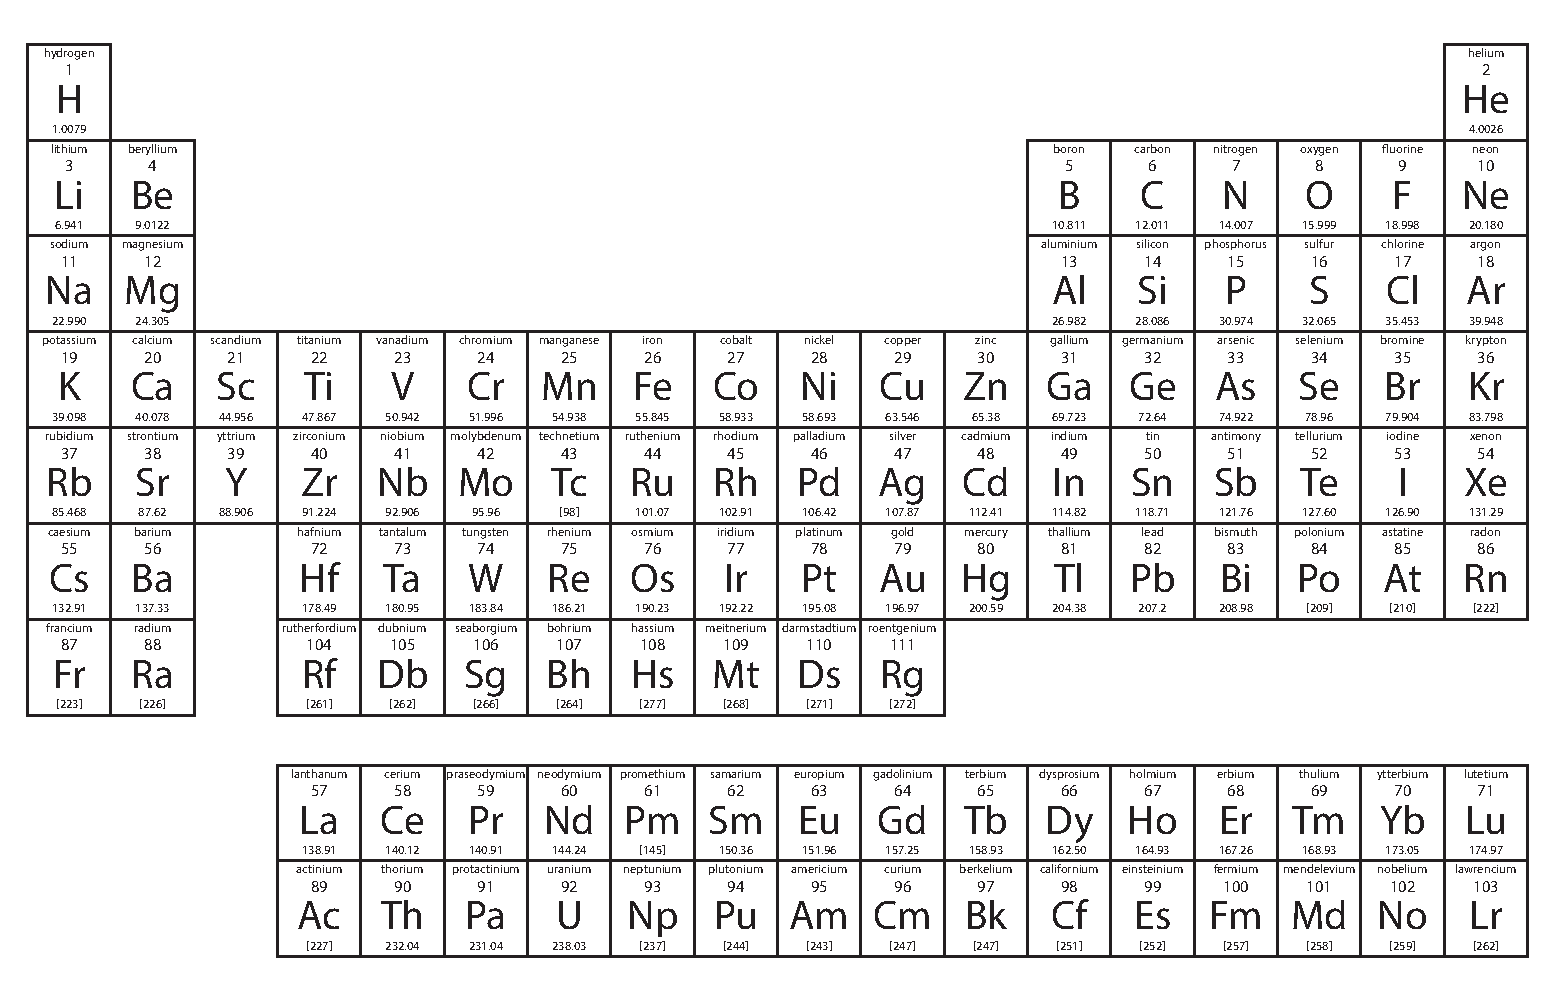
\includegraphics[scale = .8]{pertable.pdf}

\newpage
\begin{enumerate}[leftmargin = *]
\item How many atoms are in $4.0 \times 10^{-5}$ grams of Al?
\begin{enumerate}
    \item $8.9 \times 10^{17}$
    \item $2.4 \times 10^{19}$
    \item $6.5 \times 10^{20}$
    \item $2.0 \times 10^{22}$
\end{enumerate}

\item Barium chloride reacts with sodium sulfate according to the following equation:
    $$\ce{BaCl2(aq) + Na2SO4(aq) -> BaSO4(s) + 2NaCl(aq)}$$
A student mixes a solution containing 10.0 g \ce{BaCl2} ($M$ = 208.2) with a solution containing 10.0 g \ce{Na2SO4} ($M$ = 142.1) and obtains 12.0 g \ce{BaSO4} ($M$ = 233.2). What is the percent yield of this reaction.
\begin{enumerate}
\item 60.0\%
\item 73.1 \%
\item 93.3 \%
\item The isolated barium sulfate is most likely wet, since the yield would otherwise be greater than 100\%
\end{enumerate}
\item A 5.73 g sample of a liquid hydrocarbon burned in excess oxygen produces 17.48 g \ce{CO2}. What is the formula of the hydrocarbon?
\begin{enumerate}
    \item \ce{C5H12}
    \item \ce{C6H6}
    \item \ce{C6H10}
    \item \ce{C6H12}
\end{enumerate}
\item A student determined the density of a solid to be 2.90, 2.91, and 2.93 g cm$^{-3}$. If the actual density of this solid is 2.70 g cm$^{-3}$, how should the student's results be described?
\begin{enumerate}
    \item high accuracy and high precision
    \item low accuracy and high precision
    \item high accuracy and low precision
    \item low accuracy and low precision
\end{enumerate}
\item A flame test was performed to confirm the identity of a
metal ion in solution. The result was a green flame.
Which of the following metal ions is indicated? 
 \begin{enumerate}
     \item copper
     \item sodium
     \item strontium
     \item zinc
 \end{enumerate}
 \newpage
 \item Which of the following is a weak electrolyte in aqueous
solution?
\begin{enumerate}
    \item \ce{HF}
    \item \ce{NaF}
    \item \ce{HCl}
    \item \ce{KCl}
\end{enumerate}
\item A sample of He gas in a flexible container at room
temperature exhibits a certain pressure. What will be the
new pressure when the absolute temperature and volume
of the container are both halved? The pressure of the He
will be
\begin{enumerate}
    \item the same
    \item doubled
    \item halved
    \item quadrupled
\end{enumerate}
\item A gas mixture at 27 $^{\circ}$ C and 1 atm contains equal masses
of He, \ce{H2}, \ce{CO2}, and \ce{CH4}. How do their molecular
velocities compare?
\begin{enumerate}
    \item \ce{He} = \ce{H2} = \ce{CO2} = \ce{CH4}
    \item \ce{He} < \ce{H2} < \ce{CO2} < \ce{CH4} 
    \item \ce{H2}  < \ce{He} < \ce{CH4} < \ce{CO2}
    \item \ce{CO2} < \ce{CH4} < \ce{He} < \ce{H2}
\end{enumerate}
\item The molecules in a sample of pure liquid dichloromethane, \ce{CH2Cl2}, experience which of the following intermolecular forces?
\begin{enumerate}[I]
    \item dispersion forces
    \item dipole-dipole forces
    \item hydrogen bonding
\end{enumerate}
\begin{enumerate}
    \item I only
    \item II only
    \item I and II only
    \item I, II, III
\end{enumerate}
\item The standard enthalpy of formationn for \ce{NH3}(g) \SI{-46.1}{\kilo\joule\per\mole}. Calculate $\Delta{H}\standard$ for the reaction: 
\begin{align*}
    \ce{2NH3(g) -> N2(g) + 3H2(g)}
\end{align*}
\begin{enumerate}
    \item \SI{-92.2}{\kilo\joule}
    \item \SI{-46.1}{\kilo\joule}
    \item \SI{46.1}{\kilo\joule}
    \item \SI{92.2}{\kilo\joule}
\end{enumerate}
\newpage
\item Which is a statement of the Second Law of Thermodynamics?
\begin{enumerate}
    \item The energy of the universe is conserved.
    \item The energy of the universe is decreasing.
    \item The entropy of the universe is conserved.
    \item The entropy of the universe is increasing.
\end{enumerate}
\item A gold ring that weighs 3.81 g is heated to \SI{84.0}{\celsius} and placed in \SI{50.0}{\gram} of \ce{H2O} at \SI{22.1}{\celsius}. What is the final temperature?
\begin{enumerate}
    \item \SI{22.2}{\celsius}
    \item \SI{24.0}{\celsius}
    \item \SI{26.5}{\celsius}
    \item \SI{53.1}{\celsius}
\end{enumerate}
\item The activation energy for a reaction can be determined by measuring the reaction rate at different 
\begin{enumerate}
    \item temperatures.
    \item catalyst concentrations.
    \item reactant concentrations.
    \item times on the reaction curve.
\end{enumerate}
\item A catalyst speeds up a chemical reaction by
\begin{enumerate}
    \item shifting the equilibrium.
    \item increasing the activation energy.
    \item decreasing the reaction enthalpy.
    \item providing an alternate reaction pathway.
\end{enumerate}
\item For the reaction:
\begin{align*}
    \ce{(CH3)3CBr(aq) + OH-(aq) -> (CH3)3COH(aq) + Br-(aq)}
\end{align*}
it is found that halving the concentration of \ce{(CH3)3CBr} causes the reaction rate to be halved but halving the concentration of \ce{OH-} has no effect on the rate. What is the rate law?
\begin{enumerate}
    \item Rate  = $k\left[\ce{(CH3)3CBr}\right]^{\frac{1}{2}}\left[\ce{OH-}\right]$
   \item Rate  = $k\left[\ce{(CH3)3CBr}\right]^{2}\left[\ce{OH-}\right]$
   \item Rate  = $k\left[\ce{(CH3)3CBr}\right]^{\frac{1}{2}}$
   \item Rate  = $k\left[\ce{(CH3)3CBr}\right]$
\end{enumerate}
\item What is the pH of a 0.0015 M solution of \ce{HNO3}?
\begin{enumerate}
    \item 1.41
    \item 2.82
    \item 5.65
    \item 11.18
\end{enumerate}
\newpage
\item In a solution of formic acid ($K_a = 1.7 \times 10^{-4}$), the $[\ce{H+}] = 2.3 \times 10^{-3}$. What is the concentration of formic acid in \si{\mole\per\liter}?
\begin{enumerate}
    \item $7.2 \times 10 ^{-2}$
    \item $3.1\times 10^{-2}$
    \item $5.3 \times 10^{-6}$
    \item $3.9 \times 10^{-7}$
\end{enumerate}
\item For the equilibrium system:
\begin{align*}
    \ce{CO(g) + 2H2(g) <=> CH3COH(l)}
\end{align*}
what is $K_c$?
\begin{align}
K_c = \frac{[\ce{CH3OH}]}{2[\ce{CO}][\ce{H2}]} \\
K_c = \frac{[\ce{CH3OH}]}{[\ce{CO}][\ce{H2}]^2} \\
K_c = \frac{1}{2[\ce{CO}][\ce{H2}]} \\
K_c = \frac{1}{[\ce{CO}][\ce{H2}]^2} 
\end{align}
\item Which change represents an oxidation
\begin{enumerate}
    \item \ce{NO2- -> N2}
    \item \ce{VO^2+ -> VO3-}
    \item \ce{ClO- -> Cl-}
    \item \ce{CrO4^2- -> Cr2O7^2-}
\end{enumerate}
\item Which is a consistent set of values for a specific redox reaction carried out under standard conditions?

{
\renewcommand{\arraystretch}{1.5}
\begin{tabular}{lllll}
  & $E\standard$ & $\Delta{G\standard}$ & Description &  \\
(a) &  +  &  $-$  &       spontaneous        &  \\
(b) &  $-$  &  +  &       spontaneous        &  \\
(c) &  +  &  +  &       nonspontaneous     &  \\
(d) &  $-$ &  $-$  &       nonspontaneous
\end{tabular}
}
\item For a galvanic cell involving the half-reactions at standard conditions,
\begin{align*}
    \ce{Au^3+ + 3e- -> Au} && &E\standard = \SI{1.50}{\volt} \\
    \ce{Tl+ e- -> Tl} && &E\standard = \SI{-0.34}{\volt}
\end{align*}
what is $E\standard_{cell}$?
\begin{enumerate}
    \item \SI{0.48}{\volt}
    \item \SI{1.16}{\volt}
    \item \SI{1.84}{\volt}
    \item \SI{2.52}{\volt} 
\end{enumerate}
\item Which set of quantam numbers is not possible?
\begin{enumerate}
    \item $n = 2$, $l = 1$, $m_l = +1$, $m_s = -\frac{1}{2}$
    \item $n = 3$, $l = 2$, $m_l = +1$, $m_s = +\frac{1}{2}$
    \item $n = 4$, $l = 4$, $m_l = -1$, $m_s = +\frac{1}{2}$
    \item $n = 5$, $l = 2$, $m_l = 2$, $m_s = -\frac{1}{2}$
\end{enumerate}
\item In which list are the ions arranged in order of decreasing
size?
\begin{enumerate}
    \item \ce{S^2-, Br-, K+, Ca^2+}
    \item \ce{Br-, S^2-, K+, Ca^2+}
    \item \ce{K+, Ca^2+, S^2-, Br-}
    \item \ce{Ca^2+, K+, S^2-, Br-}
\end{enumerate}
\item The removal of an electron from which gaseous atom requires the greatest amount of energy?
\begin{enumerate}
    \item Na
    \item Cl
    \item K
    \item Br
\end{enumerate}
\item Which ionic solid has the greatest lattice energy?
\begin{enumerate}
    \item NaCl
    \item MgO
    \item KBr
    \item SrS
\end{enumerate}
\item What is the shape of the \ce{ClF3} molecule?
\begin{enumerate}
    \item trigonal planar
    \item trigonal pyramidal
    \item T-shaped
    \item tetrahedral
\end{enumerate}
\item Which molecule has no permanent dipole moment?
\begin{enumerate}
    \item \ce{BCl3}
    \item \ce{NCl3}
    \item \ce{CHCl3}
    \item \ce{PCl3}
\end{enumerate}
\end{enumerate}
\begin{center}
    \LARGE\textbf{END OF TEST}
\end{center}

\end{document}
